\documentclass{standalone}
\usepackage{tikz}

\begin{document}

	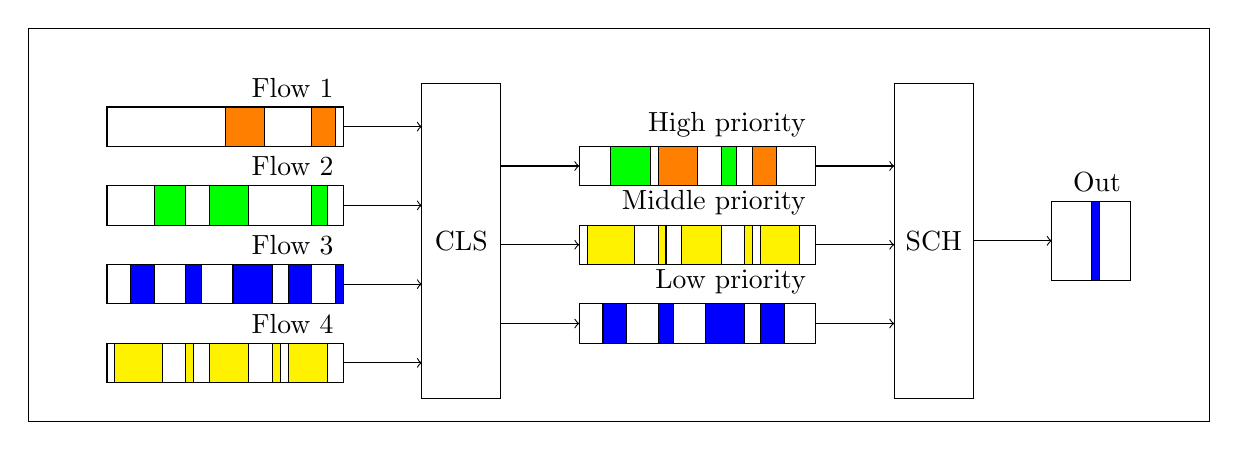
\begin{tikzpicture}
A		\draw (0, 0) rectangle (15, 5);

		% Flow 1
		\draw (1, 3.5) rectangle (4, 4) node[above left] {Flow 1};
		\draw[fill=orange] (2.5,   3.5) rectangle (3,   4);
		\draw[fill=orange] (3.6, 3.5) rectangle (3.9, 4);

		% Flow 2
		\draw (1, 2.5) rectangle (4, 3) node[above left] {Flow 2};
		\draw[fill=green] (1.6,   2.5) rectangle (2,   3);
		\draw[fill=green] (2.3, 2.5) rectangle (2.8, 3);
		\draw[fill=green] (3.6, 2.5) rectangle (3.8, 3);

		% Flow 3
		\draw (1, 1.5) rectangle (4, 2) node[above left] {Flow 3};
		\draw[fill=blue] (1.3, 1.5) rectangle (1.6, 2);
		\draw[fill=blue] (2,   1.5) rectangle (2.2, 2);
		\draw[fill=blue] (2.6, 1.5) rectangle (3.1, 2);
		\draw[fill=blue] (3.3, 1.5) rectangle (3.6, 2);
		\draw[fill=blue] (3.9, 1.5) rectangle (4, 2);


		% Flow 4
		\draw (1, 0.5) rectangle (4, 1) node[above left] {Flow 4};
		\draw[fill=yellow] (1.1, 0.5) rectangle (1.7, 1);
		\draw[fill=yellow] (2,   0.5) rectangle (2.1, 1);
		\draw[fill=yellow] (2.3, 0.5) rectangle (2.8, 1);
		\draw[fill=yellow] (3.1, 0.5) rectangle (3.2, 1);
		\draw[fill=yellow] (3.3, 0.5) rectangle (3.8, 1);

		% Classifier
		\draw (5,0.3) rectangle (6, 4.3) node[pos=.5] {CLS};

		\draw[->] (4, 3.75) to (5, 3.75);
		\draw[->] (4, 2.75) to (5, 2.75);
		\draw[->] (4, 1.75) to (5, 1.75);
		\draw[->] (4, 0.75) to (5, 0.75);

		\draw[->] (6, 1.25) to (7, 1.25);
		\draw[->] (6, 2.25) to (7, 2.25);
		\draw[->] (6, 3.25) to (7, 3.25);

		%Low
		\draw[fill=blue] (7.3,  1) rectangle (7.6,  1.5);
		\draw[fill=blue] (8,    1) rectangle (8.2,  1.5);
		\draw[fill=blue] (8.6,  1) rectangle (9.1, 1.5);
		\draw[fill=blue] (9.3, 1) rectangle  (9.6, 1.5);
		\draw (7, 1) rectangle (10,1.5) node[above left] {Low priority};

		% Middle
		\draw[fill=yellow] (7.1, 2) rectangle  (7.7, 2.5);
		\draw[fill=yellow] (8,   2) rectangle (8.1, 2.5);
		\draw[fill=yellow] (8.3, 2) rectangle (8.8, 2.5);
		\draw[fill=yellow] (9.1, 2) rectangle (9.2, 2.5);
		\draw[fill=yellow] (9.3, 2) rectangle (9.8, 2.5);

		\draw (7, 2) rectangle (10,2.5) node[above left] {Middle priority};

		% High

		\draw[fill=orange] (9.2,   3) rectangle (9.5, 3.5);
		\draw[fill=green]  (8.8, 3) rectangle   (9, 3.5);
		\draw[fill=orange] (8,   3) rectangle   (8.5, 3.5);
		\draw[fill=green]  (7.4,  3) rectangle  (7.9,  3.5);

		\draw (7, 3) rectangle (10,3.5) node[above left] {High priority};

		% Shed
		\draw[->] (10, 1.25) to (11, 1.25);
		\draw[->] (10, 2.25) to (11, 2.25);
		\draw[->] (10, 3.25) to (11, 3.25);

		\draw (11,0.3) rectangle (12, 4.3) node[pos=.5] {SCH};

		% Out
		\draw (13, 1.8) rectangle (14, 2.8) node[above left] {Out};
		\draw[fill=blue] (13.5, 1.8) rectangle (13.6, 2.8);

		\draw[->] (12, 2.3) to (13, 2.3);

	\end{tikzpicture}

\end{document}
